\documentclass[12pt]{article}
\usepackage{graphicx,amssymb,amsmath,subfigure}

\oddsidemargin  -0.5 cm
\evensidemargin 0.0 cm
\textwidth      6.5in
\headheight     0.0in
\topmargin      -1 cm
\textheight=9in

\renewcommand{\arraystretch}{1.25}

\title{Global Alignment of the CMS Muon System \\ using a Track-Based Algorithm}
\author{Jim Pivarski, Alexei Safonov, Karoly Banicz, Riccardo Bellan}

\begin{document}
\maketitle
\begin{abstract}
It will have an abstract.  Scope of the paper: baseline HIP procedure
for barrel and endcap, CSC overlaps procedure for endcap.  Methods
described in full detail, results from a 50~pb$^{-1}$ Monte Carlo
study with the major systematic effects, results from CRAFT alignment
(global muon only or global muon plus stand-alone? depends on time
available), independent cross-checks, and 50--200~pb$^{-1}$ prediction
for muon momentum resolution.  It will back up a much shorter public
paper.  Completed in this version: everything except results and
conclusions (sections 4, 5, and 7).
\end{abstract}
\pagebreak

\tableofcontents
\pagebreak

\section{Introduction}

The CMS experiment features a large muon tracking system which will
likely be essential for early LHC discoveries.  As with all tracking
systems, the resolution of its reconstructed tracks depends on two
main components:
\begin{itemize}
\item intrinsic hit resolution, or how precisely the intersection of
  passing particles with its measurement planes can be determined for
  individual tracks, and
\item alignment, or how accurately the position of the measurement
  planes are known in 3-D space, affecting all tracks.
\end{itemize}
These components combine in quadrature, so track resolution can be
expected to improve significantly until the alignment is much better
than the intrinsic resolution, which is about 200--300~$\mu$m for the
CMS muon system.  Therefore, our baseline goal for the 2009--2010
physics run is to align the muon system to this level of accuracy.

Though this 44-layer muon system can act as a tracking system on its
own, it was designed to operate in conjunction with the other CMS
subsystems, particularly the inner silicon tracker.  Together, the two
tracking subsystems form a global tracking system with high intrinsic
hit resolution in the tracker and large lever arm in the muon system
(particularly important for high-$p_T$ tracks; $1/p_T$ resolution
scales with lever arm squared).  Above $p_T \gtrsim 200$~GeV in the
barrel and 1~TeV in the endcap, the inclusion of muon system hits
significantly improves muon resolution over a tracker-only measurement
(Fig~\ref{fig:tdr_muon_resolution}).  Muon alignment is therefore
important for any physics analysis featuring high-$p_T$ muons, such as
$Z' \to \mu\mu$ and $W' \to \mu\nu$, but it is also important for
analyses that use the muon system as an independent check on the
tracker, such as the search for heavy stable charged particles, which
verifies velocity from tracker $dE/dx$ with muon barrel timing
(equivalent to spatial resolution).

\begin{figure}[hb]
\begin{center} \includegraphics[width=0.35\linewidth]{Figure_001-005-a.pdf} \hspace{0.5 cm} \includegraphics[width=0.35\linewidth]{Figure_001-005-b.pdf} \end{center}
\caption{Momentum resolution of the inner tracker, muon system, and combined system, as a function of $p_T$ and $\eta$.  (Source: Physics TDR~\cite{tdr}) \label{fig:tdr_muon_resolution}}
\end{figure}

To obtain high-quality global muon tracks, the tracker and muon system
must be aligned in the same coordinate system.  We choose to define
the global coordinate system as the inner tracker's system and verify
that it is stable for each block of runs.  This is convenient because
the low-momentum tracks used to measure the alignment (20--100~GeV)
are best determined by the tracker.  If a sudden movement or slow
drift is observed, we have the necessary machinery to redefine the
global coordinate system in a more neutral way.

There are several independent ways to measure alignment, all of which
are actively being pursued.  Alignment with global tracks provides a
simple way to link distant subdetector elements and is sensitive to
exactly the same parameters as the final physics object: the global
muon itself.  For example, if misalignment perpendicular to the
measurement plane of a layer cannot be determined from a large sample
of tracks, then it also does not distort the physics resolution of
muons in the same sized sample.  Alignment with local tracks, such as
linear track stubs through pairs of neighboring detector elements, can
determine the relative positions of those elements and provide both an
early (low statistics) alignment measurement and a powerful
cross-check on the global alignment, as local tracks are much less
sensitive to propagation errors and can correlate measurements in
different combinations than the global method.  The CMS muon system is
also instrumented with a network of physical measurement devices such
as lasers, calipers, and inclinometers, which provide another
independent measurement of detector alignment, free from any tracking
errors but requiring a careful propagtion of cumulative measurements.
This paper will focus on alignment with global tracks for both the
barrel and the endcap, and demonstrate an alignment procedure with
local tracks in the endcap.

\subsection{Geometry of the muon system}

The muon system contains three basic types of tracking chambers: drift
tube (DT) chambers in the barrel, cathode strip chambers (CSC) in the
endcap, and resistive plate chambers (RPC) in both.  The chambers are
modular tracking detectors, 1--4~m each, whose internal geometry is
well understood from production tests.  They are mounted on 15~m tall
barrel wheels and endcap disks which serve to compactly return the
solenoid's magnetic field and also filter all particles except for
muons.  The position and orientation of each chamber is allowed to
slip under the influence of the 3.8~T CMS solenoid, rather than
distort the chambers non-rigidly.  In the center of the endcap, the
distortion can be as large as 1.4~cm.

This paper focuses on algorithms to align the DT chambers and CSCs as
rigid bodies whose internal geometry is assumed to be known.  The DT
internal geometry has been thoroughly studied
elsewhere \cite{internal_dt}, and a method to align CSC layers will be
described in section~\ref{sec:CSC_layer_alignment}.  The RPCs are used
primarily for triggering with a resolution of 1--2~cm, so they don't
contribute to muon resolution and don't need to be aligned.

The chambers are grouped in stations (loosely by distance from the
interaction point), wheels/disks (modular transverse slices), and
sectors/chambers (azimuthal divisions).  Table~\ref{tab:geometry} presents an
overview of this structure, and Fig~\ref{fig:muon_system_labeled}
shows where the stations are located in CMS.

\begin{table}
\caption{Geographical organization of muon chambers. \label{tab:geometry}}
\begin{center}
\begin{tabular}{c | c}
Barrel & Endcap \\\hline
\renewcommand{\arraystretch}{2.5}
\begin{tabular}{p{0.08\linewidth} p{0.125\linewidth} p{0.13\linewidth}}
wheels & $-2$ to $+2$ & physically moveable transverse slices \\
stations & MB1 to 4 & cylinders of fixed radius from beamline \\
sectors & 1--12 \mbox{(1--14 in} station~4) & \raggedright $\phi=0$ is sector 1, increasing counter-clockwise \\
\end{tabular} &
\begin{tabular}{p{0.1\linewidth} p{0.125\linewidth} p{0.14\linewidth}}
endcaps & $-$ and $+$ & forward and backward halves \\
disks & ME1 to 4 & physically moveable transverse slices \\
rings \mbox{(stations)} & \raggedright 1/1ab, 1/2, 1/3, 2/1, 2/2, 3/1, 3/2, 4/1 & rings of fixed radius from beamline \\
chambers & 1--36 \raggedright \mbox{(1--18 in} 2/1, 3/1, 4/1) & \raggedright $\phi=0$ is sector 1, increasing counter-clockwise \\
\end{tabular}
\vspace{-1 cm}
\end{tabular}
\end{center}
\end{table}

\begin{figure}
\hspace{-1.3 cm} \includegraphics[width=1.2\linewidth]{muon_system_labeled.pdf}

\caption{A quarter-view of CMS with labeled muon barrel (MB) and endcap (ME) stations. \label{fig:muon_system_labeled}}
\end{figure}

In barrel stations 1--3, DT chambers contain superlayers which measure
orthogonal directions: superlayers~1 and 3 measure the muon distance
of closest approach in the transverse plane, while superlayer~2
measures the longitudinal closest approach, parallel with the
beamline.  Barrel station~4 chambers have no superlayer~2, so they are
one-dimensional devices.  Each chamber has a local coordinate system,
where local $x$ is the coordinate superlayers~1 and 3 measure, local
$y$ is the coordinate superlayer~2 measures, and local $z$ is
orthogonal to the measurement plane.  By contrast, the global $x$
coordinate is the horizontal distance from the beamline, global $y$ is
vertical, and global $z$ is parallel to the beamline, roughly
coinciding with the DT local $y$.  The goal of alignment can be
restated as a very careful determination of the transformation
functions between the local coordinate systems and the global system.

In the CSCs, cathode strips fan radially from the beamline,
intersected by anode wires.  We define the same sort of local
coordinate system in the CSCs, with local $x$ being the direction
measured mostly by strips, local $y$ as the direction measured by
wires, and local $z$ perpendicular to the measurement plane, roughly
corresponding with global $z$.  Table~\ref{tab:local_coordinates}
summarizes the coordinate systems.

\begin{table}
\caption{Definitions and correspondance of coordinate systems. \label{tab:local_coordinates}}
\begin{center}
\begin{tabular}{c | c | c}
Global frame & Local DT frames & Local CSC frames \\\hline
\begin{tabular}{c p{0.2\linewidth}}
$x$ & horizontal, toward center of LHC \\
$y$ & vertical, up \\
$z$ & along beamline \\
origin & nominal interaction point \\
$r\phi$ & combination of $x$ and $y$ perpendicular to
rays from the beamline
\end{tabular} &
\begin{tabular}{c p{0.2\linewidth}}
$x$ & superlayer~1 and 3 measurement, roughly global $r\phi$ \\
$y$ & superlayer~2 measurement, roughly global $z$ \\
$z$ & out of plane, roughly radial from beamline \\
origin & center of chamber
\end{tabular} &
\begin{tabular}{c p{0.2\linewidth}}
$x$ & strip measurement, roughly global $r\phi$ \\
$y$ & wire measurement, roughly radial from beamline \\
$z$ & out of plane, roughly global $z$ \\
origin & center of chamber
\end{tabular}
\end{tabular}

\vspace{0.25 cm}
$\phi_x$, $\phi_y$, and $\phi_z$ are rotation angles around local
coordinate axes.

\end{center}
\end{table}

\section{Description of the global alignment algorithm}

The basic idea is to accumulate high-$p_T$ muons which pass through
two regions: a well-aligned reference volume, usually the silicon
tracker, and the target volume under study.  Muon tracks are fitted
using information from the reference only, and alignables in the
target (muon chambers, layers, wheels, or disks) are translated and
rotated to minimize the difference between muon tracks and muon hits
(residuals).

This procedure can be seen as an extreme limit of the HIP algorithm
used to align the silicon tracker, in which tracks are fitted in a
single tracking volume with large uncertainties in the positions of
the alignables, which reduces the sensitivity of the final track fits
to outlying alignables.  Outlying alignables tend to have larger
residuals, which are used to pull them toward their rightful positions
with repeated applications of the procedure.

In comparison with the silicon tracker alignment case, however,
individual tracks propagated through the muon system are much less
trustworthy due to the large amounts of material they must penetrate.
Muons, particularly low-momentum muons, can be highly deflected by the
single and multiple scattering which occurs unpredictably in dense
material, and can distort the track-fit if not recognized by the
algorithm.  Since our track-fitting algorithm properly includes such
scattering, a direct application of the tracker alignment procedure
would lead to overzealous application of scattering by the
track-fitting algorithm: the displacement of muon hits in misaligned
chambers would be overcorrected by a scattering assumption, and thus
adversely affect all or most of the tracks in the sample.  By freely
propagating muon tracks from the reference volume through the target
volume, and not allowing the muon hits to bias the propagated track,
only the muons that actually do scatter significantly are useless for
alignment.

The technique is particularly useful when the reference volume is the
silicon tracker, since the tracker dominates the precision of track
parameters for the muons used in alignment ($20 < p_T < 100$~GeV).
The disadvantage is that any distortions in the tracker geometry,
which can persist after completing tracker alignment if the $\chi^2$
of its tracks are invariant under such transformations, would be
extrapolated to the muon system, distorting the muon geometry in the
same way.  However, the broad track angle distribution of cosmic rays
allows us to observe residuals on tracks from different parts of the
reference volume, and therefore put bounds on the bias from the track
source.  The tracker alignment procedure uses this same technique to
constrain its ``weak modes,'' but the muon system provides additional
checks with a longer lever arm, to amplify the errors and more easily
notice the effects.

It's also a computationally useful feature that excluding target hits
from the track-fit eliminates the coupling between track-fitting and
alignment.  We therefore do not need to iterate the procedure, as in
the case in the tracker-HIP alignment, because geometry updates in the
target have no effect on track-fitting in the reference.  In the
language of MillePede-based algorithms, the matrix of alignment
parameters and track parameters becomes block-diagonal, greatly
simplifying its inversion and eliminating the fundamental distinction
between the HIP and MillePede approaches.

\subsection{Alignment datasets and track-fitting procedures}

Data for muon HIP alignment are derived from three main sources: LHC
collisions, cosmic rays that pass through the tracker, and all cosmic
rays (relaxing tracker-pointing increases the sample by an order of
magnitude).  The main difference is in their orientations: collisions
muons originate strictly in the interaction point at the center of CMS
and are nearly symmetric in $\phi$ and charge, while cosmic rays are
more broadly distributed in entrance angles, though steeply peaked
toward the vertical, with 30\% more $\mu^+$ than $\mu^-$.  It should
be noted that all collisions muons which reach a given chamber pass
through approximately the same region of the tracker, and can
therefore be sensitive to local errors in the tracker alignment, while
cosmic rays are only sensitive to global distortions in the tracker.
The distinction between tracker-pointing and non-tracker-pointing
cosmic rays is important because only the former can use the tracker
as a reference.

The production mechanism of collisions muons doesn't need to be
controlled, only the $p_T$ distribution.  Whether a muon was the
product of a $b$ decay or a $Z$ decay, its propagation through the
tracker and muon system is determined solely by its momentum.  (A
future incarnation of this algorithm may take advantage of the mass
constraint from a large $Z$, $\Upsilon$, or $J/\psi$ $\to\mu\mu$ sample to reduce reference bias,
but this version doesn't.)  The influence of muons from pions decaying
in flight is minimized in the same way as highly scattered muons,
which will be described in section~\ref{sec:fitting}.  We therefore only
require one muon in the event, with 20~GeV~$<$~$p_T$~$<$~100~GeV.  The
lower limit excludes tracks that are likely to scatter and the upper
limit guarantees that track parameters are well determined by the
tracker.  This distribution is highly peaked at the low momentum end
of the spectrum, as it is dominated by QCD-related sources.

The events are collected by AlCaReco producers, which select good
muons in prompt reconstruction at CERN's Tier-0, reduce the data
streams to include only the needed tracks and hits, and send them to
the CMS CAF to be persistently stored on a local disk.  The AlCaReco
stream for collisions muons is named MuAlCalIsolatedMu (though no
isolation requirements are applied), the stream for tracker-pointing
cosmics is MuAlGlobalCosmics, and the stream for all cosmic rays is
MuAlStandAloneCosmics.\label{page:AlCaReco}

The first step in the alignment algorithm is to re-fit the tracks,
using the original track parameters to seed the new fit.  This allows
us to take advantage of any updates in the tracker geometry and to fit
global-muon tracks with artificially large errors in the muon alignable
positions.  (Global muon tracks each contain a list of associated hits
from both the tracker and the muon chambers, and have passed standard
quality requirements for matching the tracker and muon stubs to each
other.)  By imposing artificially large errors on the muon hits (a
variance of 1000~cm$^{2}$, isotropically in $x$-$y$-$z$), the new
track fit effectively ignores them, giving us the desired tracker-only
fit with the muon residuals calculated by the same subroutines as
standard track-reconstruction, to be certain that we're optimizing the
same quantity that will be used to fit tracks.  When aligning with
stand-alone muons (which have no tracker hits), we define the reference
and target volumes by setting large errors to selected chambers.
These errors are expressed in a mutable database record, so the
boundary between reference and target can be arbitrarily defined.

In performing the re-fit, it is essential that the algorithm starts
with the reference hits and ends with the target hits; otherwise, the
new track's trajectory through the target will be determined by the
old seed track, rather than a new fit to the reference.  For
collisions muons, this means that fitting must be performed in the
direction of the muon momentum (``alongMomentum'' or ``insideOut''),
and for cosmic rays, two specialized refitters,
globalCosmicMuonTrajectories and standAloneMuonTrajectories, have been
written to set the hit order in a reliable way.  The
globalCosmicMuonTrajectories algorithm arranges hits to start in the
tracker and end in the muon system, while standAloneMuonTrajectories
requires the first hit to be the closest to the center of the
detector, so that alignment knowledge can be propagated from wheel~0
out to the endcaps.

\subsection{Calculation of super-residuals}
\label{sec:super_residuals}

As a tracking volume, the muon system is highly structured.  Inside of
each chamber, muons encounter very little material, and in the barrel
chambers, very little magnetic field.  Muon hits are therefore more
highly correlated with their neighbors in the same chamber than they
are with propagated tracks.

If we ignore this fact, we would misrepresent the statistical
resolution of the alignment result.  For the sake of argument,
consider an extreme case in which residuals in an $N$-layer chamber
are 100\% correlated with each other.  If we accumulate a histogram of
residuals for that chamber, each track will yield the same result $N$
times, though the distribution would be wide because of uncertainties
in track propagation.  If we then compute the mean of that
distribution or fit it, the reported uncertainties would be a factor
of $\sqrt{N}$ too small.

Instead, we combine all residuals on one track in one chamber into a
single super-residual; each super-residual is an independent
measurement.  We compute a super-residual from the constant term in a
linear fit of residuals $\Delta x_i$ as a function of local $z$, the
coordinate perpendicular to the chamber's layer planes.  Non-zero
slopes in $\Delta x(z)$ are either caused by errors in the track's
local trajectory or by rotations of the chamber (around $z=0$).  The
constant term from this fitting method is more representative of the
chamber's overall residual than a mean of $\Delta x_i$ would be,
because the hits are not necessarily symmetric around the chamber
center in $z$, especially if hit inefficiencies or weighting are
allowed (see Fig~\ref{fig:superresidual0}).  The linear fit is
computed analytically, with weights from intrinsic hit uncertainties
($\sigma_i$).

\begin{figure}
\begin{center} 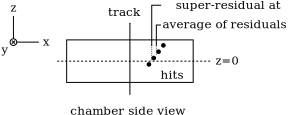
\includegraphics{superresidual0.pdf} \end{center}
\caption{A super-residual is the constant from a linear fit to residuals vs.\ local $z$, and is therefore a better measure of the ``residual at chamber center'' than the average of residuals. \label{fig:superresidual0}}
\end{figure}

\begin{eqnarray}
\mbox{constant} &=& \frac{1}{\mbox{denominator}} \left(\sum\frac{z_i^2}{\sigma_i^2} \sum\frac{\Delta x_i}{\sigma_i^2} - \sum\frac{z_i}{\sigma_i^2} \sum\frac{z_i \Delta x_i}{\sigma_i^2}\right) \\
\mbox{slope} &=& \frac{1}{\mbox{denominator}} \left(\sum\frac{1}{\sigma_i^2} \sum\frac{z_i \Delta x_i}{\sigma_i^2} - \sum\frac{z_i}{\sigma_i^2} \sum\frac{\Delta x_i}{\sigma_i^2}\right) \\
\mbox{where denominator} &=& \sum\frac{1}{\sigma_i^2} \sum\frac{z_i^2}{\sigma_i^2} - \left(\sum\frac{z_i}{\sigma_i^2}\right)^2
\end{eqnarray}

Barrel DT chambers measure two coordinates, local $x$ and $y$, but
with disjoint sets of hits.  Hits in superlayers~1 and 3 measure the
local $x$ coordinate (approximately global $r\phi$) but not $y$, while
hits in superlayer~2 measure local $y$ (parallel with the beamline)
but not $x$.  We therefore treat these as two independent systems and
compute one super-residual for superlayers~1 and 3 and another
super-residual for superlayer~2.

Endcap CSCs also measure two coordinates using different systems---
cathode strips and anode wires--- though they do not decompose into an
orthogonal, rectilinear coordinate system.  Strips measure $r\phi$,
the curvilinear coordinate which is always perpendicular to rays from
the beamline, while wires measure $y$ or a linear combination of $x$
and $y$, depending on the station.  The wire measurement is not useful
for alignment because its granularity is much larger than the
alignment precision, ?? to 5~cm.  (One could use edges in hit
efficiency to determine $y$, but that's beyond the scope of this
paper.)  Using only strips, it is most convenient to compute $r\phi$
super-residuals and apply alignment corrections in $r\phi$, rather
than the CSCs' local $x$ coordinates (Fig~\ref{fig:csc_localrphi}).
Other than its interpretation, CSC $r\phi$ super-residuals are treated
the same way as DT $x$ super-residuals in alignment fits.

\begin{figure}
\begin{center} 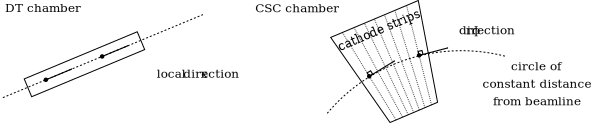
\includegraphics{strip_direction.pdf} \end{center}
\caption{Local $x$ and $y$ coordinates in DT chambers are rectilinear, but the fanning of CSC strips makes it more convenient to measure residuals and align CSCs in curvilinear $r\phi$. \label{fig:csc_localrphi}}
\end{figure}

By combining hit information into one or two measurements per chamber,
super-residuals are similar to, but not exactly the same as 2-D
segment residuals, the distance and angular difference between a track
and a linear fit to the hits in the chamber.  The distinction is that
segment residuals assume that the muon's propagation through the
chamber is linear, while super-residuals only assume that the growth
of error between the true and reconstructed paths is linear.  The
actual path of a muon may be significantly non-linear in ME1/1 and
ME1/2, which contain 2.5~T and 1.0~T fields inside the gas volumes,
respectively.  Super-residuals represent deviations in these chambers
with more precision than a segment residual would.

\subsection{Fitting the super-residuals distribution}
\label{sec:fitting}

Once a large set of super-residuals has been collected for each
chamber, its alignment correction is computed from the mode of its
distribution.  The mode is to be preferred over the mean and
the median because the alignment signal has a background which is not
guaranteed to be symmetric.

Each super-residual can be thought of as a single track's notion of
where the chamber is, and the combined measurement should be
determined from the most popular answer.  Muons that scatter or are
misrepresentative because they're actually from pion decays-in-flight
divide their votes among a continuum of wrong answers, while good
muons with minimal scattering agree on a single answer, with some
Gaussian smearing.  The distribution of residuals from scattering
depends on the distribution of material in front of the chamber and
the angles of the tracks used for alignment, which need not be
symmetric at a given point in the detector.  This asymmetry would skew
an average of the super-residuals distribution, but it has much less
impact on the peak position.

To determine the mode of a distribution from a random sample, one must
fit it with an ansatz of known mode.  The physical scattering
processes generally have power-law distributions and the extrapolation
of a trajectory from experimental measurements smears the peak of
nearly zero scattering into a Gaussian bell-curve (see
Fig~\ref{fig:residuals_barrel}).  These effects are best represented
by a convolution:
\begin{figure}
\begin{center} \includegraphics[width=0.4\linewidth]{residuals_barrel.pdf} \end{center}
\caption{Super-residuals distributions have a central Gaussian core from unscattered muons and power-law tails from scattered muons. This is demonstrated by taking advantage of the fact that scattering is highly correlated with $p_T$. \label{fig:residuals_barrel}}
\end{figure}
\begin{equation}
f(\Delta x; x_0, \sigma, \Gamma) = \int_{-\infty}^\infty
\frac{1}{\pi}\frac{\Gamma/2}{(\Delta x - \xi - x_0)^2 + (\Gamma/2)^2} \times 
\frac{1}{\sqrt{2\pi} \sigma} \exp\left(\frac{-\xi^2}{2 \sigma^2}\right) \, d\xi
\label{eqn:fitfunction}
\end{equation}
where $x_0$ is the mode of the residuals $\{\Delta x_i\}$, $\sigma$ is
the experimental resolution and $\Gamma$ is the full width at half
maximum of a Cauchy-Lorentz distribution, chosen for its power-law
tails and simplicity.  This ansatz does not describe the scattering
background in detail, as the real distribution might scale with a
different power and the Cauchy-Lorentz distribution isn't asymmetric,
but it absorbs much of the background and allows the Gaussian part to
more accurately fit the peak (see Fig~\ref{fig:fitfunction}).

\begin{figure}
\begin{center} \includegraphics[width=0.4\linewidth]{fitfunction.pdf} \end{center}
\caption{Fit function for residuals with a Gaussian core and power-law tails.  The residuals in this plot were selected from a geographically small region of the detector (within DT~station~4, wheel~0) to avoid smearing from misalignment, and the fit was performed without binning. \label{fig:fitfunction}}
\end{figure}

We fit Eqn~\ref{eqn:fitfunction} to the super-residuals of each
chamber with an unbinned maximum likelihood method to handle
low-statistics cases well and to avoid dependence on bin width.  It
should be noted that a simple average ($\sum \Delta x_i/N$) is equal
to the mode of an unbinned Gaussian fit, so while this algorithm may
be procedurally much more complicated, it is functionally a small
modification from just using the mean.  Outlying residuals contribute
much less to the log-likelihood of $f$ than they would to the
log-likelihood of a Gaussian tail, and hence they have much less
influence on the fitted value of $x_0$, regardless of whether they're
symmetrically distributed or not.  We also reject any residual beyond
10~meters of zero or 10~standard deviations of the mean for
robustness against nonsense input.

For computational efficiency, Eqn~\ref{eqn:fitfunction} is
pre-computed in bins of $\sigma$ and $\Gamma$.  Bilinear
interpolations from the look-up table have been verified up to
$|\Delta x| < 100 \, \sigma$ and $\Gamma < 10 \, \sigma$.  If the
MINUIT fit settles upon a value outside of this table, it is treated
as a fit failure.

This procedure was developed to manage asymmetric residuals from
scattering.  The CMSSW track propagator computes appropriate error
ellipses for multiple scattering when it propagates through dense
material, but our method of de-weighting hits in the target volume by
inflating chamber position uncertainties washes out that information,
so we won't be able to use it the way the tracker HIP algorithm does.
Also, if we were to rely on the propagator's estimate of scattering,
rather than fitting it in the data, our algorithm would depend on the
track reconstruction's assumed material budget, which might be wrong.

\subsection{Determining alignment parameters from fits}
\label{sec:alignment_from_fits}

We collect $x$ and $y$ super-residuals from each DT chamber and
$r\phi$ super-residuals from each CSC, so determining only the peak of
each distribution would only allow us to align DT chambers in two
dimensions and CSCs in one.  We want to align as many of the 6 rigid
body degrees of freedom as possible, and fortunately, we can access
most of the others by identifying trends in the residuals
distributions.

Consider a chamber rotated around its local $z$ axis, as shown in
Fig~\ref{fig:phiz}.  This $\phi_z$ rotation creates discrepancies
between tracks and their hits at the edges of the detector, but not in
the center.  For small misalignments ($\sin\phi_z \approx \phi_z$),
the $\Delta x$ residual is proportional to the $y$ position of the
impact point, and the $\Delta y$ residual is proportional to the $x$
position of the impact point, with the constant of proportionality in
both cases being $\phi_z$.

\begin{figure}
\begin{center} 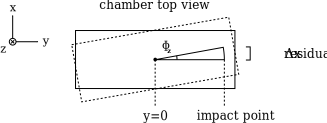
\includegraphics{phiz_diagram.pdf} \end{center}
\caption{If the chamber is rotated in its layer plane ($\phi_z$ misalignment), the crest of the $\Delta x$ residuals distribution will vary with $y$ impact point as $\Delta x = \sin \phi_z \cdot y$ or $\Delta x \approx \phi_z \, y$.  We include $\phi_z$ as a free parameter in the fit to perform this alignment, simultaneously with $\delta x$.  The same holds for $\Delta y$ residuals and the $x$ impact point.  \label{fig:phiz}}
\end{figure}

We can extract $\delta x$ and $\phi_z$ alignment corrections from a
collection of superlayer~1 and 3 super-residuals by fitting the
distribution to a straight line; a fit to $\delta y$ and $\phi_z$ in
the superlayer~2 super-residuals allows us to cross-check $\phi_z$
from an independent dataset.  A discrepancy between the two $\phi_z$
fits would indicate a problem with the chamber geometry description.
In a future version of the algorithm, when this validity has been
fully established, we can use the higher-precision superlayer~1 and 3
$\phi_z$ result to improve the accuracy of superlayer~2 fits for
$\delta y$.  It is important for the fits to either know the correct
$\phi_z$ value or fit for it, because an incorrect $\phi_z$ would bias
$\delta x$ or $\delta y$ if the distribution of muons across the
surface of the chamber is asymmetric.

Linear fits are included in the residuals fit described in
section~\ref{sec:fitting} by expanding the $x_0$ parameter
(Eqn~\ref{eqn:fitfunction}) into an expression involving two
parameters.  To determine $\delta_x$ and $\phi_z$ alignment
corrections, we expand $f$ to
\begin{equation}
f_x(\Delta x, y_{\mbox{\scriptsize impact}}; \delta_x, \phi_z, \sigma, \Gamma) \mbox{ with } (\delta_x + y_{\mbox{\scriptsize impact}} \, \phi_z) \mbox{ replacing } x_0 \label{eqn:first_correction}
\end{equation}
and for $\delta_y$ and $\delta_{\phi_z}$, we use
\begin{equation}
f_y(\Delta y, x_{\mbox{\scriptsize impact}}; \delta_y, \phi_z, \sigma, \Gamma) \mbox{ with } (\delta_y + x_{\mbox{\scriptsize impact}} \, \phi_z) \mbox{ replacing } x_0 \mbox{.}
\end{equation}
In both cases, the impact point is taken from the track
extrapolation, rather than the hits themselves.  (Not all chambers
have enough information to determine the impact point in both
dimensions, and it doesn't need to be known with high precision.)

Next, consider a chamber which has been misaligned in the local $z$
direction, as shown in Fig~\ref{fig:zpos_a}.  The offset introduces
$\Delta x$ and $\Delta y$ residuals for angled tracks, proportional to
the $dx/dz$ and $dy/dz$ angles, respectively.  We can compute the
$\delta z$ alignment correction by adding this dependence to the fit
as well.
\begin{figure}
\subfigure[Linear relationship between $\Delta x$ residuals, $\delta z$ misalignment, and $dx/dz$ track angle: \mbox{$\Delta x = (dx/dz) \, \delta z$}]{\begin{minipage}{0.4\linewidth} \begin{center} 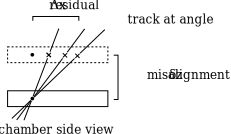
\includegraphics{zpos_diagram.pdf} \end{center} \vspace{0.2 cm} \end{minipage} \label{fig:zpos_a}} \hfill \subfigure[Correlation between $x$ impact point and $dx/dz$ track angle for tracks that pass close to the origin]{\begin{minipage}{0.4\linewidth} \begin{center} 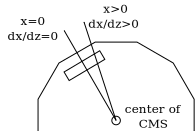
\includegraphics{trackangle_correlation.pdf} \end{center} \vspace{0.2 cm} \end{minipage} \label{fig:zpos_b}}
\caption{Misalignments perpendicular to the measurement plane (local $z$) are included in the fit as a linear trend with respect to track entrance angle (which is often correlated with impact point).  The same holds for $\Delta y$ residuals and the $dy/dz$ track entrance angle. \label{fig:zpos}}
\end{figure}
\begin{eqnarray}
&& f_{xz}(\Delta x, y_{\mbox{\scriptsize impact}}, \tfrac{dx}{dz}; \delta_x, \phi_z, \delta_z, \sigma, \Gamma) \mbox{ with } x_0 \to (\delta_x + y_{\mbox{\scriptsize impact}} \, \phi_z + \tfrac{dx}{dz} \, \delta_z) \\
&& f_{yz}(\Delta y, x_{\mbox{\scriptsize impact}}, \tfrac{dy}{dz}; \delta_y, \phi_z, \delta_z, \sigma, \Gamma) \mbox{ with } x_0 \to (\delta_y + x_{\mbox{\scriptsize impact}} \, \phi_z + \tfrac{dy}{dz} \, \delta_z) \label{eqn:dydz_extrapolation} \label{eqn:last_correction}
\end{eqnarray}
In the superlayer~2 case, however, the distribution of muon
$\tfrac{dy}{dz}$ entrance angles is highly asymmetric, which would
make Eqn~\ref{eqn:dydz_extrapolation} a long-baseline extrapolation.
We therefore only fit for $\delta_z$ in superlayer~1\&3 and the CSCs,
and in a future version of the algorithm, the superlayer~1\&3 result
would be used to improve superlayer~2 accuracy.

To measure $\phi_z$, we had to look at $\Delta x$ residuals as a
function of $y_{\mbox{\scriptsize impact}}$, and to measure $\delta
z$, we had to look at the same residuals as a function of $dx/dz$.
Note that $dx/dz$ is correlated with $x_{\mbox{\scriptsize impact}}$
(Fig~\ref{fig:zpos_b}), especially for muons from the collision point.
(Similarly for $\Delta y$, $x_{\mbox{\scriptsize impact}}$, and
$y_{\mbox{\scriptsize impact}}$.)  If we think of $dx/dz$ as being
equivalent to $x_{\mbox{\scriptsize impact}}$, we have used all of the
spatial information available to us, and have only determined
$\delta_x$, $\delta_y$, $\delta_z$ (two ways), and $\phi_z$ (two ways).

To get the $\phi_x$ and $\phi_y$ angles, we go back to the
super-residuals and note that the slope of the linear fit to
individual hit residuals versus $z$ yields a difference in angle
between the track and the hits.  As can be seen in
Fig~\ref{fig:superresid_slope}, the $dx/dz$ slope of a super-residual
is $\tan\phi_y$, where $\phi_y$ is the angle between the track's
direction and the direction suggested by the hits.  Approximating
these as small angles, we take the super-residual $dx/dz$ slopes to be
$\phi_y$ residuals and $dy/dz$ slopes to be $\phi_x$ residuals, and
fit them to Eqn~\ref{eqn:fitfunction}.
\begin{figure}
\begin{center} 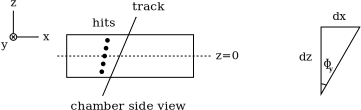
\includegraphics{superresidual.pdf} \end{center}
\caption{Super-residuals have both a value at the chamber center and a slope.  The $dx/dz$ slopes are used to align $\phi_y$ and the $dy/dz$ slopes (where available) align $\phi_x$. \label{fig:superresid_slope}}
\end{figure}

It is necessary to control the $\phi_x$ and $\phi_y$ alignment
corrections for impact point, or else $\phi_z$ misalignments will
appear as spurious $\phi_x$ and $\phi_y$ corrections when the track
source is asymmetric in entrance angle and position.  This is a fully
3-dimensional effect, diagrammed as well as possible in
Fig~\ref{fig:motivation_for_angle_controls}.  To account for this, we
add $x$ and $y$ impact point corrections to the fit function,
analogous to
Eqns~\ref{eqn:first_correction}-\ref{eqn:last_correction}.

\begin{figure}
\begin{center} 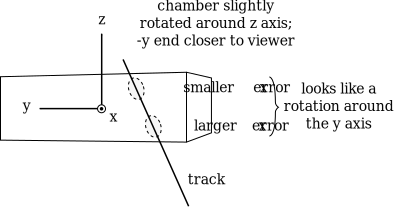
\includegraphics[width=0.6\linewidth]{motivation_for_angle_controls.pdf} \end{center}
\caption{A 3-dimensional effect in which $\phi_z$ misalignments can masquerade as $\phi_y$ misalignments when the track source is asymmetric in $dx/dz$ entrance angle and $y$ impact point.  The same is true for $\phi_x$ misalignments, swapping all $x \leftrightarrow y$. \label{fig:motivation_for_angle_controls}}
\end{figure}

The fact that scattering occurs in localized regions of the detector
introduces a strong correlation between super-residual positions and
their angles, illustrated in Fig~\ref{fig:sawtooth_diagram}.
Disagreement between a track's direction and the direction suggested
by its hits is a good indication that the muon has been scattered.  We
take advantage of this relationship to improve precision in the
$\delta x$ and $\delta y$ measurements in three ways:
\begin{figure}
\begin{center} 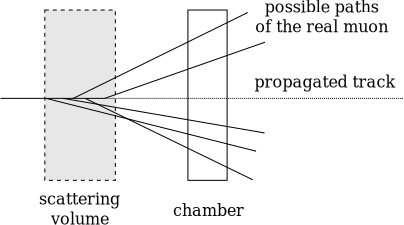
\includegraphics[height=4.5 cm]{sawtooth_diagram.pdf} \end{center}
\caption{Correlation between super-residual position error and angle error. \label{fig:sawtooth_diagram}}
\end{figure}
\begin{itemize}
\item include the average $\Delta x$ vs.~$\phi_y$ and $\Delta y$
  vs.~$\phi_x$ trends as slope parameters in the fits,
\item select only super-residuals that have slopes in a well-behaved
  linear region around zero (5~mrad in superlayer~1\&3 and CSCs,
  30~mrad in superlayer~2), and
\item use the measured $\phi_y$ or $\phi_x$ alignment to correct
  $\delta_x$ and $\delta_y$, respectively.
\end{itemize}
Depending on the location of the chamber, accounting for this
correlation improves the fitted precision by as much as a factor of~2.
The algorithm can be improved further by identifying and correcting
any other large correlations in the shape of the residuals
distributions: there is some evidence that superlayer~2 residuals and
station~1, wheels~$\pm$2 are imperfectly represented.

Table~\ref{tab:parameters} summarizes the fits and alignment
parameters for each chamber.

\begin{figure}
\begin{center}
\begin{tabular}{c}

Fits to DT superlayers~1 and 3 super-residuals \\
\begin{tabular}{| c | c |}
\hline fit to $\Delta x$ residuals & fit to $\phi_y$ residuals \\\hline
$\delta x$: peak of the distribution, independent of impact & $\phi_y$ peak of the distribution \\
$\delta z$: dependence of the peak on $dx/dz$ track angle & \\
$\phi_z$: dependence of the peak on $y$ impact point & \\
$\sigma$, $\Gamma$: width of the distribution & $\sigma$, $\Gamma$: width of the distribution \\
slope of $\Delta x$ vs.~$\phi_y$: model scattering & \\\hline
\end{tabular} \\
\\
Fits to DT superlayer~2 super-residuals \\
\begin{tabular}{| c | c |}
\hline fit to $\Delta y$ residuals & fit to $\phi_x$ residuals \\\hline
$\delta y$: peak of the distribution, independent of impact & $\phi_x$ peak of the distribution \\
$\phi_z$: dependence of the peak on $x$ impact point & \\
$\sigma$, $\Gamma$: width of the distribution & $\sigma$, $\Gamma$: width of the distribution \\
slope of $\Delta y$ vs.~$\phi_x$: model scattering & \\\hline
\end{tabular} \\
\\
Fits to CSC super-residuals \\
\begin{tabular}{| c | c |}
\hline fit to $\Delta r\phi$ residuals & fit to $\phi_y$ residuals \\\hline
$r\delta\phi$: peak of the distribution, independent of impact & $\phi_y$ peak of the distribution \\
$\delta z$: dependence of the peak on $d(r\phi)/dz$ track angle & \\
$\phi_z$: dependence of the peak on $y$ impact point & \\
$\sigma$, $\Gamma$: width of the distribution & $\sigma$, $\Gamma$: width of the distribution \\
slope of $\Delta x$ vs.~$\phi_y$: model scattering & \\\hline
\end{tabular} \\
\\
Accessible parameters \\
\begin{tabular}{c | c c c c c c}
\hline DT & \hspace{0.6 cm}$\delta_x$\hspace{0.6 cm} & $\delta_y$ & $\delta_z$ & $\phi_x$ & \hspace{0.6 cm}$\phi_y$\hspace{0.6 cm} & $\phi_z$ (two ways) \\
CSC & $\delta_x$ & inaccessible & $\delta_z$ & inaccessible & $\phi_y$ & $\phi_z$ \\
\end{tabular}
\end{tabular}

\end{center}
\caption{The six independent fits needed to align one DT chamber and one CSC. \label{tab:parameters}}
\end{figure}

\subsection{Accomodating errors in magnetic field and material budget}
\label{sec:bfield_errors}

Early in commissioning, track propagation through CMS may suffer from
poor knowledge of the magnetic field map and material budget.  This
would result in incorrect residuals and potentially a wrong alignment.
Since alignment is itself a commissioning task, it must be made
independent of any propagation errors.  Magnetic field and $dE/dx$
errors from an incorrect material budget can be identified by their
distinctive dependencies on momentum, and can both be cancelled by
taking advantage of the fact that they affect residuals in a
charge-antisymmetric way.

\begin{figure}
\subfigure[Diagram for derivation: $x$ is the displacement between straight and helical propagation of a track with radius of curvature $R$ at a distance $\ell$ from the interaction point.  If the field is mis-modelled, it would contribute $\Delta x = x_{\mbox{\scriptsize track}} - x_{\mbox{\scriptsize muon}}$ to the residual, the difference of two helical propagations with different radii.]{\begin{minipage}{0.45\linewidth} \includegraphics{bfield_diagram.pdf} \vspace{0.5 cm} \end{minipage}} \hfill \subfigure[Derivation of residuals dependence on $q/p_T$ if the magnetic field is mis-modelled.  If the $B_z$ error is also non-uniform, the above holds with ``$\Delta B_z$'' being a (non-trivial) quantity derived from field error along the track's path.]{\begin{minipage}{0.45\linewidth}
\vspace{0.7 cm}
Displacement from straight propagation:
\begin{eqnarray*}
x &=& R \left(1 - \cos\left(\sin^{-1}\left(\ell/R\right)\right)\right) \\
x &\approx& R \left(\frac{1}{2} \left(\ell/R\right)^2\right) = \frac{\ell^2}{2 R} \\
\end{eqnarray*}

\vspace{-0.2 cm}
Relationship to magnetic field $B_z$:
\[ R = \frac{\ell^2}{2 x} = \mbox{300 cm T/GeV } \frac{p_T}{q B_z} \]

Residuals from field error $\Delta B_z$:

\[ \hspace{-1 cm}\Delta x = \frac{\ell^2}{2 \cdot \mbox{300 cm T/GeV}} \, \left(\frac{q}{p_T}\right) \, \Delta B_z\hspace{-1 cm} \]

\vspace{0.1 cm}
\end{minipage}}
\caption{If the $z$ component of the magnetic field is poorly understood at the time of alignment, the error it contributes to residuals would be proportional to $q/p_T$. \label{fig:bfield}}
\end{figure}

Fig~\ref{fig:bfield} derives the effect of $B_z$ (axial) errors on
super-residuals, which is proportional to $q/p_T$ but not a simple
function of the actual $\Delta B_z$ error.  A similar derivation would
reveal that residuals from $B_r$ (radial) errors are proportional to
$q/p_z$ (Fig~\ref{fig:bfield_components}).

\begin{figure}
\begin{center}
\begin{tabular}{p{0.3\linewidth} c p{0.65\linewidth}}
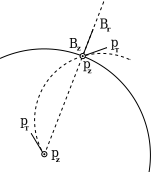
\includegraphics[width=\linewidth]{bfield_components.pdf} & \hspace{0.5 cm} &
\begin{minipage}{\linewidth}
\vspace{-4.5 cm}
\noindent Components affecting $r\phi$ and $\phi_y$ residuals:
\begin{itemize}
\item $|\vec{p}_T \times \vec{B}_z| = |\vec{p}_T| \, |\vec{B}_z|$, always normal to trajectory
\item $|\vec{p}_z \times \vec{B}_r| = |\vec{p}_z| \, |\vec{B}_r|$, approximately normal to trajectory at high momentum
\end{itemize}

\vspace{0.3 cm}
\noindent Components affecting $z$ and $\phi_x$ residuals:
\begin{itemize}
\item $p_T \times B_r$, negligible at high momentum
\end{itemize}

\end{minipage} \\
\end{tabular}
\end{center}
\caption{A summary of magnetic field components which affect residuals. \label{fig:bfield_components}}
\end{figure}

As an aside, note that the dependence of super-residuals slopes such
as $\phi_y$ on $q/p_T$ and $q/p_z$ is also bilinear, but easier to
interpret as measureable errors in the $\Delta B_z$ and $\Delta B_r$
components (Fig~\ref{fig:superresid_bfield}).  This is because the
cumulative effect that $\vec{B}$ errors have on the angle of a track
is simply the integral over its path, while the effect on residuals is
a double-integral.  Magnetic field errors can therefore be measured
directly with tracks, using an extension of the $\phi_y$ chamber angle
measurement.

\begin{figure}
\subfigure[Track angles are deflected $\phi = \sin^{-1} \ell/R \approx \ell/R$ relative to a straight-line propagation.  If the magnetic field is mis-modelled, it would add \mbox{$\Delta \phi = \phi_{\mbox{\scriptsize track}} - \phi_{\mbox{\scriptsize muon}}$} to the super-residual slope.]{\begin{minipage}{0.45\linewidth} 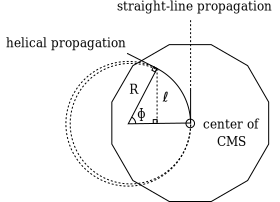
\includegraphics{bfieldangle_diagram.pdf} \vspace{0.2 cm} \end{minipage}} \hfill \subfigure[Derivation of super-residual angle in the presence of mis-modelled $B_z$.  If non-uniform, ``$\Delta B_z$'' is a simple average of magnetic field error along the track's path.]{\begin{minipage}{0.45\linewidth}
\vspace{1.75 cm}
\begin{eqnarray*}
R = \frac{\ell}{\phi} &=& \mbox{300 cm T/GeV } \frac{p_T}{q B_z} \\
\Delta \phi &=& \frac{\ell}{\mbox{300 cm T/GeV}} \left(\frac{q}{p_T}\right) \Delta B_z
\end{eqnarray*}

\vspace{1.75 cm}
\end{minipage}}
\caption{Magnetic field errors would also affect super-residual slopes.  \label{fig:superresid_bfield}}
\end{figure}

Residuals from $dE/dx$ errors have a different momentum dependence,
but the same dependence on charge.  In the momentum range of interest,
the energy muons lose in material is independent of momentum: about
2~MeV~cm$^2$/g, or 1.6~GeV/m through iron.  The track propagator
accounts for known material, so only errors in the material budget
contribute to residuals.  Energy loss affects all three components of
the track's momentum equally, so the $\theta$ angle of the track's
trajectory ($\tan\theta = p_T/p_z$) is unchanged.  The $\Delta x$ and
$\Delta \phi$ super-residuals scale in the following ways:
\begin{eqnarray}
\Delta x &\propto& \ell^2 \, q B_z \, \left(\frac{1}{p_T} - \frac{1}{p_T - \cos\theta \, dE/dx}\right) \\
\Delta \phi &\propto& \ell \, q B_z \, \left(\frac{1}{p_T} - \frac{1}{p_T - \cos\theta \, dE/dx}\right) \mbox{.}
\end{eqnarray}
which is approximately quadratic:
\begin{equation}
\frac{\frac{1}{p_1} - \frac{1}{p_1 - \Delta}}{\frac{1}{p_2} - \frac{1}{p_2 - \Delta}}
% = \frac{p_2}{p_1} \, \frac{\left(1 - \frac{1}{1 - \Delta/p_1}\right)}{\left(1 - \Delta/p_2\right)}
= \frac{p_2}{p_1} \, \frac{1 - \left(1 - \frac{\Delta}{p_1}\right)^{-1}}{1 - \left(1 - \frac{\Delta}{p_2}\right)^{-1}}
\approx \frac{p_2}{p_1} \, \frac{1 - \left(1 + \frac{\Delta}{p_1}\right)}{1 - \left(1 + \frac{\Delta}{p_2}\right)}
= \left(\frac{p_2}{p_1}\right)^2
\end{equation}

In principle, we could determine alignment corrections, magnetic field
errors, and $dE/dx$ errors all at once by adding linear and quadratic
terms to our fit function.  However, that would unnecessarily reduce
the statistical precision of our alignment measurement, especially if
propagation errors are small.  Instead, we note that both types of
propagation errors are antisymmetric with charge: positive and
negative tracks would be deflected in opposite directions (opposite
sign in the residuals contribution) by either effect
(Fig~\ref{fig:antisymmetric_bfield}).  If we compute all of our
alignment corrections from positively-charged tracks and again with
negatively-charged tracks, the charge-antisymmetric effects would
cancel in the average (Fig~\ref{fig:demo_residual}), assuming that the
positive and negative muons have the same momentum distributions
(Fig~\ref{fig:demo_momentum}).  We therefore apply the following
``two-bin'' method to calculate all alignment constants:
\begin{enumerate}
\item Separate the data into two bins by charge.
\item Compute all alignment corrections for each bin separately ($R_+$ and $R_-$).
\item Average the two to obtain final alignment results: $\dfrac{R_+ + R_-}{2}$.
\item Compute a maximally-affected quantity to trace the errors: $\dfrac{R_+ - R_-}{2}$.
\end{enumerate}

\begin{figure}
\mbox{ } \hfill \subfigure[Both $\vec{B}$ and $dE/dx$ errors affect postive and negative muons in opposite ways.]{\begin{minipage}{4 cm} \vspace{-4 cm} \mbox{ } \hfill 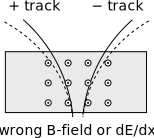
\includegraphics[width=3.5 cm]{antisymmetric_bfield.pdf} \hfill \mbox{ } \end{minipage} \label{fig:antisymmetric_bfield}}
\hfill \subfigure[The two effects depend on momentum, but are still antisymmetric for charges in a given momentum bin.]{\includegraphics[width=4 cm]{demo_residual.pdf} \label{fig:demo_residual}}
\hfill \subfigure[The momentum spectra for the two charges are proportional (cosmic rays shown above).]{\includegraphics[width=4 cm]{demo_momentum.pdf} \label{fig:demo_momentum}} \hfill \mbox{ }
% \mbox{ } \hfill \begin{minipage}{3.5 cm}\vspace{-5.3 cm}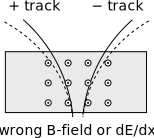
\includegraphics[width=\linewidth]{antisymmetric_bfield.pdf} \end{minipage} \hfill \hfill \includegraphics[height=5.5 cm]{demo_momentum.pdf} \hfill \includegraphics[height=5.5 cm]{demo_residual.pdf} \hfill \mbox{ }
\caption{The two-bin method for cancelling $\vec{B}$ and $dE/dx$ errors: compute corrections separately for positive muons and negative muons, then average the two results. \label{fig:twobin_method}}
\end{figure}

The systematic error after applying this procedure is a small fraction
of the error tracer; its exact value depends on how many muons are
placed in the wrong bin due to charge confusion and the degree to
which the shapes of the spectra differ for the two charges.  This
quantity is also useful for finding problematic regions of the
detector.

Positive and negative cosmic rays are known to have proportional
spectra in our momentum range of interest: the charge ratio of cosmic
secondaries is flat as a function of momentum.  Most collisions muons
should also have this property, as $b$ and $\bar{b}$ are produced in
equal abundance.  Muons from $W$ bosons may be asymmetric because
$W^+$ and $W^-$ are produced with different rates in $pp$ colliders,
but it is likely that the $\vec{B}$ and $dE/dx$ issues will be
resolved before we're fortunate enough to enrich our muon sample with
$W$ decays (by raising the $p_T$ cut).

Fig~\ref{fig:twobin_robust} demonstrates the robustness of the
two-bin method in cosmic rays: a correction in the magnetic field map
adjusts error tracer values, but not alignment residuals from the
averaging technique.

\begin{figure}
\mbox{ } \hfill \includegraphics[height=7 cm]{robustness_alignment1.pdf} \hfill
\includegraphics[height=7 cm]{robustness_errortracer2.pdf} \hfill \mbox{ }
\caption{Alignment residuals and the error tracer before and after a correction to the magnetic field map (in DT~station~4 with cosmic rays).  The alignment residuals are unaffected by the large change in magnetic field values (20--30\%). \label{fig:twobin_robust}}
\end{figure}

\section{Monitoring Tools and Validation/Verification}

Visual monitoring of the alignment procedure is useful for two
purposes: validation and verification.  By ``validation,'' we mean
simply checking that the procedure is valid, that it centers residuals
distributions as intended.  We will reserve the word ``verification''
for measurements that independently determine whether the aligned
chamber positions accord with reality.  If, for instance, tracks are
distorted by a systematic effect other than alignment, validation
procedures would pass, because they, too, are affected, but
verification procedures would not.

A generic example of validation would be to simply run the alignment
procedure twice with the same tracks: if the second alignment yields
zero corrections, then it validates the first alignment.  One way to
actually verify the aligned positions would be to select three
tracking volumes, $A$, $B$, and $C$, where $A$ is used as a reference
to align $B$ and $C$, then $B$ is used as a reference to align $C$
with a different distribution of tracks.  If the two procedures agree
about the position of $C$, then $C$'s result has been independently
verified as a real position in space.

Verification procedures do not need to be completely independent to be
useful.  As long as they contain some new information that is
systematically distinct from the alignment procedure itself, they can
add confidence to the measurement.  Monitorable quantities range from
pure validation to pure verification, and it will be important to keep
in mind roughly how much new information each observable is giving us.

This section will focus on monitoring methods and show example plots,
created under different circumstances, not necessarily the final
alignment.  For summary plots of alignment results, see
sections~\ref{sec:mcstudy} and \ref{sec:craft}.  We only show a
representative subsample of the detailed plots (which are by necessity
numerous), while the summary plots contain the complete results.

\subsection{Comparison of geometries in the database}

Our first validation tool merely checks to see if geometry
descriptions in the conditions database differ, and by how much.  It
is actually a program which converts database records into
human-readable XML files and a library for plotting geometrically
relevant differences in pyROOT.  The conversion can be reversed: the
same XML descriptions can be uploaded to the database as muon
alignments for track-reconstruction.  The features of this system are
all documented on its own twiki page:
SWGuideMuonGeometryConversion~\cite{SWGuideMuonGeometryConversion}.

In this note, we use the conversion tool to prepare test-pattern and
randomized misalignment scenarios for the Monte Carlo study, and to
plot differences in chamber parameters with respect to ideal.

\subsection{Validating residuals fits}

Our alignment fits are multi-parameter over a multi-dimensional space,
which is in principle dangerous.  The fitter has a large space in
which to find an unphysical minimum, and multi-dimensional data is
hard to visualize quantitatively.  However, our fit function has a
shape that can easily be unfolded and plotted on a 2-dimensional page.
The full fit function is a bell curve (Eqn~\ref{eqn:fitfunction}) with
the peak ($x_0$) being a multi-linear function of several variables:
$\delta_x$ (constant), $\phi_z$ (slope with respect to position $y$),
$\delta_z$ (slope with respect to entrance angle $dx/dz$), and a
control parameter for scattering (slope with respect to
super-residual slopes $\Delta \phi_y$).  The multi-linear part can be
regarded as a set of corrections to the peak position, which follows a
line in $(y, dx/dz, \Delta \phi_y)$ space, like the crest of a
mountain ridge.

To best understand the shape of the bell curve, we plot the residuals
distribution with $y$, $dx/dz$, and $\Delta \phi_y$ corrections
applied to the data.  The fit width parameters $\sigma$ and $\Gamma$
apply to this corrected curve.  We also overlay the raw distribution,
which is in general wider, but usually not visibly so.  (The residuals
distribution is much wider than any of the three peak corrections.)
Plots like this are in the first column of Fig~\ref{fig:residualsfit}.

\begin{figure}
\hspace{0.5 cm} \includegraphics[height=0.8\linewidth, angle=90]{exampleDT_rphi.pdf}

\hfill \includegraphics[height=0.8\linewidth, angle=90]{exampleDT_z.pdf} \hspace{0.5 cm}

\hspace{0.5 cm} \includegraphics[height=0.8\linewidth, angle=90]{exampleCSC_rphi.pdf}

\caption{Residuals fits for DT superlayers 1 and 3 (top), DT superlayer 2 (middle), and CSCs (bottom), from Monte Carlo with random misalignment.  See text for a full description. \label{fig:residualsfit}}
\end{figure}

To validate the control parameters, we draw profile plots of residuals
versus each dimension separately, with all corrections applied to the
data except the one shown.  For example, the $\phi_z$ correction
(second column in Fig~\ref{fig:residualsfit}) is shown as residuals
versus $y$, with $dx/dz$ and $\Delta \phi_y$ corrections applied to
the data.  The superimposed fit line is simply $f(y) = \delta_x +
\phi_z \, y$, the crest of the bell-curve extruded in $y$.  As
explained in section~\ref{sec:alignment_from_fits}, some parameters do
not have enough sensitivity to yield a good fit, so they have been
fixed.  They are still plotted, and thus they appear as horizontal
lines.

We control for magnetic field and $dE/dx$ errors by performing the fit
separately on positively-charged and negatively-charged muons, and
averaging the results.  The $\mu^+$ fits are shown in the top row of
plots in Fig~\ref{fig:residualsfit}, while the $\mu^-$ fits are in
the bottom row.  A vertical line through the bell curve shows the
average, so if track propagation is affected by an error which is
antisymmetric in charge, the two bell curves would move away from the
vertical line in opposite directions.

It is possible to visually inspect hundreds of fit functions on a
computer screen, but more difficult to peruse them in published form.
We therefore treat these as diagnostic plots, scanning through them in
early alignments for safety and producing them on demand for
suspicious fits.  In all of the Monte Carlo and real-data alignments
observed so far (thousands), the only fits which can be said to not
represent the distributions are the ones with very few entries (fewer
than $\sim$50).

\subsection{Muon system maps}

The fit-validation plots presented trends in residuals distributions
inside each chamber.  These trends were expected because they are
caused by misalignments.  However, if there are unexpected biases in
the tracks used for alignment, either due to tracker misalignments or
propagation errors, they would show up as trends in the residuals that
cross chamber boundaries.  To verify our expectation that residuals
are correlated within each chamber and uncorrelated outside, we plot
maps of the residuals across the whole muon system.

The measurement planes of the DT chambers lie nearly flat in $\phi$
and $z$, so these are the relevant abscissas for the map plots.  To
make sure that no more than one chamber corresponds to each bin in the
plots, the plots versus $z$ must be split by sector, the plots versus
$\phi$ must be split by wheel, and all plots must be split by station.
The endcaps have 18 rings which are one CSC thick (counting ME1/1a as
being distinct from ME1/1b), so each of these gets a separate $\phi$
plot.  The CSCs lie flat in $\phi$ and the radial direction, instead
of $z$, so the orthogonal plots are 36 radial spokes for each of the 8
disks.  Some examples are shown in Fig~\ref{fig:examplemap_rphi}.

\begin{figure}
\hspace{0.5 cm} \includegraphics[height=0.8\linewidth, angle=90]{examplemap_rphi1.pdf}

\hfill \includegraphics[height=0.8\linewidth, angle=90]{examplemap_rphi4.pdf} \hspace{0.5 cm}

\hspace{0.5 cm} \includegraphics[height=0.8\linewidth, angle=90]{examplemap_CSCrphi1.pdf}

\caption{Three maps of residuals before and after alignment in Monte Carlo: DT station 1, wheel 0 (top), station 4 wheel $+$2 (middle), and CSC ME$+$1, chamber 18 (bottom).  Chamber identities were not used to make the plots; boundaries are overlaid on the results. \label{fig:examplemap_rphi}}
\end{figure}

On each of these axes, we plot all 6 alignment results: $\delta_x$,
$\delta_y$, $\delta_z$, $\phi_x$, $\phi_y$, and $\phi_z$, as well as
the antisymmetric combination of fit results to trace
$\vec{B}(\vec{x})$ and $dE/dx$ errors.  Every bin is derived from the
full fitting procedure described in
section~\ref{sec:alignment_from_fits}, though parameters equivalent to
the binning are fixed.  (Letting the slope of residuals versus $x$
float in a dataset representing a narrow slice in $x$ would
statistically weaken all of the fit's results.)  As with the
fit-validation, there are too many plots to publish, but they are
useful for diagnostics.  An example of DT $\delta_z$ (radial
displacement) in cosmic ray data is presented in
Fig~\ref{fig:examplemap_zpos}.  This is a complicated quantity, the
slope of fits to residuals versus track entrance angle, and it shows
clear discontinuities at the chamber boundaries, indicating a real
misalignment.

\begin{figure}
\includegraphics[height=\linewidth, angle=90]{examplemap_DATAzpos.pdf}
\caption{Results of $\delta_z$ fits (radial alignment for DT chambers) as a function of global $z$ position.  Results agree within each chamber and disagree with their neighbors, indicating real radial misalignments. \label{fig:examplemap_zpos}}
\end{figure}

The muon system maps are the basis for binned-residual summary plots,
where the points in the maps are used to fill a histogram, and
therefore present all of the data on one page (trading depth for
breadth).  Such a plot is more incisive than a simple histogram of
residuals, because pre-averaging the residuals in geographically
relevant bins highlights systematic deviations from zero, rather than
hiding it under track-by-track scattering.  The width of the
binned-residual distribution depends on the size of the bins, but they
are standardized: 180 bins in $\phi$ from $-\pi$ to $\pi$, 60 bins in
$z$ from $-660$~cm to $660$~cm (for DTs), and 60 bins in radial
position, from $100$~cm to $700$~cm (for CSCs).
Fig~\ref{fig:twobin_robust} from section~\ref{sec:bfield_errors}
presented histograms of residuals binned in $z$.

\subsection{Verification with relative residuals}

The map plots provide some verification of the alignment in that they
meaningfully compare residuals from the same chamber with residuals
from neighboring chambers, and thus distinguish between distortions
related to the chamber and distortions related to the tracks.
However, they are the same residuals that were used to perform the
alignment, and are therefore not independent.

Independent sets of residuals allow us to more fully verify the
alignment by triangulation: after having aligned each chamber
individually to the tracker, we check the alignment with residuals on
tracks connecting the chambers themselves.  One way to do this re-uses
the alignment tracks, but ignores position information from the
tracker.  Consider the difference of residuals between two stations on
each track, diagrammed in Fig~\ref{fig:residuals_difference}:
\begin{figure}
\begin{center}
\includegraphics[height=7 cm]{residuals_difference.pdf} \hspace{1 cm} \includegraphics[height=7 cm]{residdiff23.pdf}
\end{center}
\caption{Relative residuals are linearly independent from the residuals used in alignment, and can therefore verify its correctness.  PLACEHOLDER!  This plot is from the old (3-parameter) CRAFT alignment.  AND it's the only one that showed (marginal) improvement--- stations 1$-$2 and 3$-$4 showed (marginal) degradation.  (We interpret the three as indicating no net change in {\it relative} positions.)  In the new plot, we'll combine all stations, since they have comparable widths. \label{fig:residuals_difference}}
\end{figure}
\begin{multline}
\mbox{residuals difference}(3, 2) = (\mbox{station 3 track impact point} - \mbox{station 3 hit position}) - \\
(\mbox{station 2 track impact point} - \mbox{station 2 hit position})\mbox{.}
\end{multline}
The tracker's position information cancels in the residuals
difference, as well as any random scattering that happens between the
tracker and station~2.  The residuals difference is therefore a
narrower distribution than absolute residuals and represents the
relative alignment of chambers in station~2 and chambers in station~3
(sector by sector).  The advantage unique to this method is that the
track retains momentum magnitude information from the tracker: it is a
curved ruler, where the appropriate curvature is determined by the
tracker's high-precision momentum measurement.  The difference can be
calculated for any pair of neighboring stations, but is difficult to
interpret for DT stations~4 and 3, because the sector boundaries in
station~4 don't line up with those in station~3.

A more extensive version of the same idea uses a set of aligned
chambers as a new reference for track-fitting and re-aligning their
neighbors.  Chambers aligned by both methods verify the technique,
though with less precision because the momentum resolution of the muon
system is not as high as the tracker.  Without collisions, this is the
only way to align some chambers in the muon system, because the
constraint requiring cosmic rays to pass through the tracker yields
very few tracks in the high $|z|$ regions of the detector.

\section{Global alignment results with collisions Monte Carlo}
\label{sec:mcstudy}

A study of alignment with 50~pb$^{-1}$ of simulated muons from QCD
(primarily $b\to\mu$, which is the majority of the muons that we'll
see).  I have the event samples in AlCaReco format, so it's ready to
go.  I've put it on hold until the tracker alignment is sufficiently
well understood for us to do a combined alignment study which will
become the new 50 and 200~pb$^{-1}$ alignment scenarios.

\subsection{Scaling with statistics}

\subsection{Dependence on tracker misalignment}

\subsection{Dependence on magnetic field errors}

\section{Global alignment results with cosmic ray data}
\label{sec:craft}

I've described all of the method and plotting techniques, so this
section will be light on text and heavy on plots with interpretations.
I'm running the alignment now, and re-running it with small changes in
the configuration to optimize our use of the data.  I'll make all of
the plots when I have a final alignment, ready to be used for
tracker-pointing re-processing.

\subsection{Validation plots}

\subsection{Verification with relative residuals}

\subsection{Verification with stand-alone muon alignments}

This will take several weeks longer than everything else.

\subsection{Verification with cosmic track splitting}

Cosmic track splitting study by Nhan Tran and Alessio Bonato applied
to global muons.  It's independent because nothing in the alignment
procedure explicitly correlated the top chambers with the bottom
chambers.  It will need to be repeated with the new alignment (as well
as the new magnetic field, new tracker alignment, and new tracker
weights).  Naturally, they'll need to be acknowledged.

\section{Relative alignment of CSCs with local tracks}

We have focused so far on global alignment because of its importance
in muon track-fitting, but local alignment methods have a different
set of advantages which can be used to improve our overall
understanding.  Locally-propagated tracks, for instance from one
chamber to its neighbor, suffer far less from propagation errors,
yielding narrower residuals distributions and fewer systematic
uncertainties.  High precision can be achieved with fewer tracks
because of the narrowness of the residuals, and the track source need
not point to the tracker, so the endcap can be aligned before first
collisions with beam-halo data.  When collisions muons are available
for the global alignment procedure, local alignment will severely test
it and provide diagnostics in the case of a disagreement.

The disadvantage of local alignment algorithms is that they do not
relate the coordinate frame of the aligned system to a common
standard.  In this section, we will describe a procedure that aligns
CSCs within rings, but does not relate the aligned rings to each other
or the tracker.  Global muons from collisions will be required to make
this connection, though we can combine residuals from all the chambers
in each ring to minimize statistical uncertainty and average over
possible systematic effects.

\subsection{Description of the CSC Overlaps algorithm}
\label{sec:overlaps_algorithm}

In the muon endcap, CSCs were designed to overlap slightly with their
neighbors for the purpose of local alignment.  In each ring except
ME1/3, tracks on the left edge of chamber~$i$ can be expected to also
pass through the right edge of chamber~$i+1$, so both chambers can
independently determine the track parameters with all 6 layers.  If
these chambers systematically disagree about the positions of tracks
in a shared coordinate system, then one or both are misaligned.
Relative alignment corrections can be propagated through the ring
until we return to the first chamber, at which point the collection of
chambers must form a consistent circle, a constraint known as closure.

This can be made more formal by defining $N$ = 18 or 36 alignment
corrections $A_i$ (where $i \in \{1\ldots 18\}$ for ME2/1, ME3/1,
ME4/1 and $i \in \{1\ldots 36\}$ for the other stations).  The ring
also has $N$ residuals distributions, but each residuals distribution
corresponds to a pair of chambers, not an individual chamber, because
each residual is the position of the track as measured in chamber~$i$
minus the position of the track as measured in chamber~$i+1$.  (Index
arithmetic should be presumed to be mod $N$, such that $i+1=1$ when
$i=N$.  Remember that the chambers are arranged in a circle.)  To use
the language of the preceeding sections in this note, we may think of
one chamber as the reference tracking volume and the other as the
target to be aligned, except that there is no reason to prefer one as
a reference above the others.  Label the mean of the residuals
distribution corresponding to chambers~$i$ and $i+1$ as
$\alpha_{i\mbox{\scriptsize, }i+1}$.  We can use the mean of the
residuals distribution, rather than a fit for its peak, because
scattering is not an issue.

If we move chambers~$i$ and $i+1$ by $A_i$ and $A_{i+1}$, the mean of
the overlap residuals can be expected to change from
$\alpha_{i\mbox{\scriptsize, }i+1}$ to
$\alpha_{i\mbox{\scriptsize, }i+1} - (A_i - A_{i+1})$.  We want to find
a complete set of corrections to minimize all of the residuals means,
so we define a $\chi^2$ as
\begin{equation}
\chi^2 = (\alpha_{12} - A_1 + A_2)^2 + (\alpha_{23} - A_2 + A_3)^2 + \ldots + (\alpha_{N1} - A_N + A_1)^2
\end{equation}
and minimize it by setting its derivatives to zero.  For example,
\begin{equation}
\frac{1}{2} \frac{\partial \chi^2}{\partial A_2} = (\alpha_{12} - A_1 + A_2) - (\alpha_{23} - A_2 + A_3) = 0 \mbox{.}
\end{equation}
The complete set of such equations, written in matrix form, looks like
the following (with $N=5$ for brevity):
\begin{equation}
\left(\begin{array}{c}
\alpha_{12} - \alpha_{51} \\
\alpha_{23} - \alpha_{12} \\
\alpha_{34} - \alpha_{23} \\
\alpha_{45} - \alpha_{34} \\
\alpha_{51} - \alpha_{45}
\end{array} \right)
=
\left(\begin{array}{r r r r r}
2 & -1 &  &  & -1 \\
-1 & 2 & -1 &  &  \\
 & -1 & 2 & -1 &  \\
 &  & -1 & 2 & -1 \\
-1 &  &  & -1 & 2
\end{array}\right)
\left(\begin{array}{c}
A_1 \\
A_2 \\
A_3 \\
A_4 \\
A_5 \\
\end{array} \right)\mbox{.}
\label{eqn:NbyNmatrix}
\end{equation}
To align all $N$ chambers, we need only invert this $N\times N$
matrix.  We did not break the symmetry between the reference system
and the target system: this procedure mutually aligns all chambers at
once (similar to the MillePede algorithm used to align the tracker,
but a much smaller computational scale: our $N \ll$ millions).

Unfortunately, the matrix in Eqn~\ref{eqn:NbyNmatrix} is singular
because a procedure like this cannot determine the global position of
the whole system.  Adding the same constant to every $A_i$, which
would rotate the whole ring rigidly, would leave the $\chi^2$
invariant because the relative positions of every pair of chambers is
unchanged by the collective motion.  Since there is a direction in
$\{A_i\}$-space in which $\chi^2$ is flat, it cannot be minimized by
setting its derivatives to zero.  One way to solve the problem is to
refuse motion in the flat direction by fixing one chamber, e.g.\ force
$A_1=0$ and make chamber~1 the reference.
\begin{equation}
\left(\begin{array}{c}
0 \\
\alpha_{23} - \alpha_{12} \\
\alpha_{34} - \alpha_{23} \\
\alpha_{45} - \alpha_{34} \\
\alpha_{51} - \alpha_{45}
\end{array} \right)
=
\left(\begin{array}{r r r r r}
1 & 0 & 0 & 0 & 0 \\
-1 & 2 & -1 &  &  \\
 & -1 & 2 & -1 &  \\
 &  & -1 & 2 & -1 \\
-1 &  &  & -1 & 2
\end{array}\right)
\left(\begin{array}{c}
A_1 \\
A_2 \\
A_3 \\
A_4 \\
A_5 \\
\end{array} \right)
\end{equation}
However, if chamber~1 is misaligned, it would take the whole ring with
it.  Ring misalignments can be corrected later with global alignment,
but it is best to avoid introducing them.  Instead, we can make the
flat direction quadratic in $\chi^2$ by preferring $\{A_i\}$ sets that
have an average of zero (minimally rotate the ring).  This can be
accomplished by adding a term like
\begin{equation}
\left[ \frac{1}{N} \left(A_1 + A_2 + \ldots + A_N\right) \right]^2
\label{eqn:average}
\end{equation}
to the $\chi^2$.  Each derivative equation becomes
\begin{equation}
\frac{1}{2} \frac{\partial \chi^2}{\partial A_i} = (\alpha_{i-1\mbox{\scriptsize, }i} - A_{i-1} + A_i) - (\alpha_{i\mbox{\scriptsize, }i+1} - A_i + A_{i+1}) + \frac{1}{N^2} \sum_{i=1}^N A_i = 0 \mbox{,}
\end{equation}
so the the matrix equation is now
\begin{equation}
\left(\begin{array}{c}
\alpha_{12} - \alpha_{51} \\
\alpha_{23} - \alpha_{12} \\
\alpha_{34} - \alpha_{23} \\
\alpha_{45} - \alpha_{34} \\
\alpha_{51} - \alpha_{45}
\end{array} \right)
=
\left[\left(\begin{array}{r r r r r}
2 & -1 &  &  & -1 \\
-1 & 2 & -1 &  &  \\
 & -1 & 2 & -1 &  \\
 &  & -1 & 2 & -1 \\
-1 &  &  & -1 & 2
\end{array}\right)
+
\frac{1}{N^2}
\left(\begin{array}{r r r r r}
1 & 1 & 1 & 1 & 1 \\
1 & 1 & 1 & 1 & 1 \\
1 & 1 & 1 & 1 & 1 \\
1 & 1 & 1 & 1 & 1 \\
1 & 1 & 1 & 1 & 1
\end{array}\right)
\right]
\left(\begin{array}{c}
A_1 \\
A_2 \\
A_3 \\
A_4 \\
A_5 \\
\end{array} \right)\mbox{.}
\label{eqn:solution}
\end{equation}
It has a unique solution in which the average correction
(Eqn~\ref{eqn:average}) minimized to exactly zero.  Actually, adding
any non-zero constant to every element would yield the same solution as
the physically-motivated $\frac{1}{N^2}$.

The circular ring of chambers also provides an internal cross-check:
the sum of the means of pairwise residuals must be zero.  If not, no
combination of alignment corrections can center all of the residuals,
because
\begin{equation}
\mbox{closure} = \sum_{i=1}^N \alpha_{i\mbox{\scriptsize, }i+1} - (A_i - A_{i+1}) = \sum_{i=1}^N \alpha_{i\mbox{\scriptsize, }i+1}
\end{equation}
is independent of $\{A_i\}$.  (Note that $\sum_{i=1}^N A_{i+1}$ is
just a reindexing of $\sum_{i=1}^N A_i$ because index arithmetic is
understood to be mod $N$.)  With non-zero closure, the solution of
Eqn~\ref{eqn:solution} uniformly distributes residuals so that they
all have non-zero means, which is to say, every chamber disagrees with
its neighbor about where the tracks are.  Unclosed $r\phi$ residuals
either imply
\begin{itemize}
\item the average distance of the chambers from the beamline is
  incorrect, or
\item the presumed width of the chambers is incorrect.
\end{itemize}
In the first case, the circumference of the ring is miscalculated
because the wrong radius is assumed; in the second case, the wrong arc
is assumed per chamber.  In the course of developing this technique,
we discovered a 15~mm closure error, which derived from an 800~$\mu$m
error in the active width of the chamber description, ultimately from
a 0.09\% error in the pitch angle of each cathode strip (10~$\mu$m per
strip).  It is a very sensitive technique!

\subsection{Local CSC alignment parameters}

As much as possible, the same techniques are used to calculate
residuals and alignment corrections in the local procedure as in the
global.  Tracks propagated to a chamber are compared with the
chamber's segment position and angle, much like the super-residuals
described in section~\ref{sec:super_residuals}.  Anode wire
measurements are ignored due to their large granularity, and strips
are taken to measure curvilinear $r\phi$ residuals, rather than
cartesian local $x$, again in direct analogy with the global
procedure.  The difference is that the source for global tracks is the
tracker, propagated through magnetic fields and many radiation lengths
of material, while local tracks are extrapolations from a linear fit
in the neighboring chamber.  To treat the pair of chambers
symmetrically, hits in each are fitted to line segments on the surface
of a cylinder around the beamline
\begin{equation}
\phi(z) = a + bz
\end{equation}
and the parameters of these two fits are compared at the plane
equidistant between the chamber centers (at $z = (z_1 + z_2)/2$, where
$z_1$ and $z_2$ are the global $z$ positions of the two chambers).

Three parameters are accessible with this technique (Fig~\ref{fig:overlaps_parameters}):
\begin{enumerate}
\item the relative
$\phi_y$ of the two chambers is their average difference in slopes ($\Delta b$),
\item the relative $\delta_{r\phi}$ position is the difference in intercepts ($\Delta
a$), and
\item the relative $\phi_z$ angle is the difference in intercepts
as a function of hit position ($d(\Delta a)/dy$).  
\end{enumerate}
These parameters are interdependent in the sense that the
$\delta_{r\phi}$ result depends on $\phi_y$ and the $\phi_z$ result
depends on $\delta_{r\phi}$, but the dependencies are unidirectional.
If corrected in the above order, first $\phi_y$, then $\delta_{r\phi}$, then
$\phi_z$, the parameters decouple, avoiding the need for a combined
fit.

\begin{figure}
\subfigure[Determination of $\phi_y$ from slopes.]{\includegraphics[width=0.35\linewidth]{topview_1.pdf}} \hfill \subfigure[Determination of $\delta_{r\phi}$ from intercepts at $z=0$.]{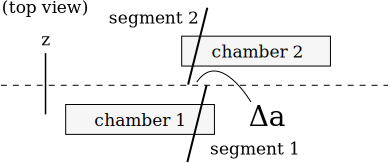
\includegraphics[width=0.35\linewidth]{topview_2.pdf}} \hfill \subfigure[Determination of $\phi_z$ from $d(\Delta a)/dy$.]{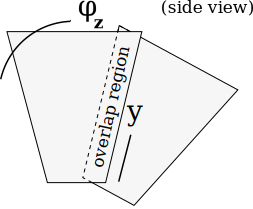
\includegraphics[width=0.2\linewidth]{sideview.pdf}}
\caption{The three alignment parameters accessible to local track matching in CSCs. \label{fig:overlaps_parameters}}
\end{figure}

The formalism developed in section~\ref{sec:overlaps_algorithm}
can be applied to each parameter separately.  First,
$\alpha_{i\mbox{\scriptsize, }i+1}$ is defined as $b_i - b_{i+1}$ and $A_i$
as ${\phi_y}_i$ to align the angles, then
$\alpha_{i\mbox{\scriptsize, }i+1}$ becomes $a_i - a_{i+1}$ and $A_i$
becomes ${\delta_{r\phi}}_i$ to align the positions, and similarly for
$\phi_z$.

\subsection{Specialized trigger and data streams}

Only events with muons that thread the narrow overlaps between
chambers are useful to this procedure, which is a small fraction of
the whole.  Beam-halo and collisions muons are equally useful, but
they come from different sources (primary datasets) because they're
reconstructed differently.  We therefore have special triggers and
data streams for each case, to avoid losing events to generic
prescales.

Four triggers are designed to accept beam-halo events.  They are
\begin{itemize}
\item HLT\_CSCBeamHalo: simply passes L1\_SingleMuBeamHalo bit, likely
  to be prescaled,
\item HLT\_CSCBeamHaloRing2or3: same but additionally requires
  reconstructed hits in ME$n$/2 or ME1/3, which are less common and
  therefore deserve a lower prescale,
\item HLT\_CSCBeamHaloOverlapsRing1 and Ring2: requires clusters of
  reconstructed hits in neighboring chambers, consistent with a muon
  in the overlap region.
\end{itemize}
Naturally, the two specialized overlaps triggers are essential to the
CSC Overlaps procedure; the others are for cross-checks and detector
studies which may be unrelated to alignment.  To produce one complete
ME$n$/1 alignment per day, we would need 0.4~Hz from
HLT\_CSCBeamHaloOverlapsRing1, and for one ME$n$/2 alignment per day,
we would need 0.8~Hz from HLT\_CSCBeamHaloOverlapsRing2 (scaling from
2008 exercise).

Events with beam-halo trigger bits are then collected by the
MuAlBeamHaloOverlaps AlCaReco stream (similar to MuAlCalIsolatedMu,
MuAlGlobalCosmics, and MuAlStandAloneCosmics, discussed on
page~\pageref{page:AlCaReco}).  MuAlBeamHaloOverlaps has no explicit
$p_T$ cut (the momentum of tracks parallel to $\vec{B}$ would not be
measured well anyway), with an option to apply a coarse energy cut by
requiring the reconstructed track to pass through a given number of
stations.

Collisions muons to be used with the CSC Overlaps procedure are
collected with the standard single-muon triggers and whatever
prescales that implies (in flux at the low end of the momentum scale).
They are then delivered to alignment via the MuAlOverlaps stream.  As
usual, the AlCaReco streams contain only what is needed for alignment:
tracks and the hits associated with those tracks, so they use very
little disk space for the number of events they contain.

\subsection{Results from the 2008 LHC run}

On September 10--17, 2008, protons circulated in the LHC tunnel,
providing a source of beam-halo muons which we used to test the CSC
Overlaps procedure.  Three-quarters of the beam-halo events were
collected from a 9-minute run on the evening of September 11 (run
number 60232; 33,000 HLT\_CSCBeamHaloOverlapsRing1 triggers).  To
guarantee a consistent snapshot of the detector geometry, we select
data from this run only.  The CSC Overlaps procedure is only
meaningful when applied to rings in which all chambers are actively
taking data; missing data in any one chamber removes two residuals
constraints (e.g.\ $\alpha_{i-1\mbox{\scriptsize, }i}$ and
$\alpha_{i\mbox{\scriptsize, }i+1}$), making Eqn~\ref{eqn:solution}
unsolvable.  In this run, ME$-$2/1 and ME$-$3/1 were the only
completely-active rings (the beam was coming from the minus side of
CMS, which contributed significantly more muons to the minus endcap).
Many of the CSC commissioning problems experienced in 2008 have been
fixed in the long shut-down, so we can expect more complete rings in
2009.

The procedure was first applied to beam-halo Monte Carlo with
approximately the same number of events but a different azimuthal and
radial distribution than the real beam.  (The azimuthal and radial
distribution of the real beam varied considerably from run to run,
more than the difference between our chosen run and the Monte Carlo.)
Fig~\ref{fig:overlaps_mc} presents the results from a simulated
alignment procedure, starting from a standard misaligned geometry
(2008 ``STARTUP'' scenario).  The standard deviation of the difference
between aligned chamber positions and MC truth quantifies the
precision of the technique, though the interpretation is approximate
because of the differences in track distribution.

\begin{figure}
\subfigure[$\phi_y$ precision is $\sim$1~mrad]{\includegraphics[width=0.3\linewidth]{mcchamber_phiy.pdf}} \hfill \subfigure[$\delta_{r\phi}$ precision is $\sim$230~$\mu$m]{\includegraphics[width=0.3\linewidth]{mcchamber_rphi.pdf}} \hfill \subfigure[$\phi_z$ precision is $\sim$0.25~mrad]{\includegraphics[width=0.3\linewidth]{mcchamber_phiz.pdf}} \hfill
\caption{Comparison of alignment parameters with MC truth before (dark) and after (light) a simulated beam-halo alignment with similar statistics to the 2008 LHC run. \label{fig:overlaps_mc}}
\end{figure}

To verify the aligned positions of chambers in real data, we compare
the beam-halo results with photogrammetry, an alignment derived from a
literal photograph of the detector.  Each chamber has two alignment
pins, connected directly to the active layer planes and capped with a
reflective disk, the center of which is accurately measured by the
photographs.  An average of the two pin positions yields the $r\phi$
location of the chamber and a difference of the two pin positions,
divided by the distance between the pins, yields the $\phi_z$ angle.
The $\phi_y$ angle is inaccessible to photogrammetry, because both
pins lie on the chamber's local $y$ axis.  The photogrammetry results
are clearly independent from the track-based results, and can
therefore be used to verify the latter.  The beam-halo data were
collected with no magnetic field, just like the photogrammetry, so we
can be confident that they describe the same geometry.

Fig~\ref{fig:overlaps_data1} presents the aligned value of each
parameter of each chamber relative to ideal values for both
track-based alignment and photogrammetry.  One can see that the two
methods are both measuring significant differences with respect to
ideal, and that the results are highly correlated.

\begin{figure}
\begin{center}
\hspace{-1.3 cm} \begin{minipage}{1.2\linewidth}
\includegraphics[height=0.45\linewidth, angle=90]{compare_m21_phiy.pdf} \includegraphics[height=0.45\linewidth, angle=90]{compare_m31_phiy.pdf}

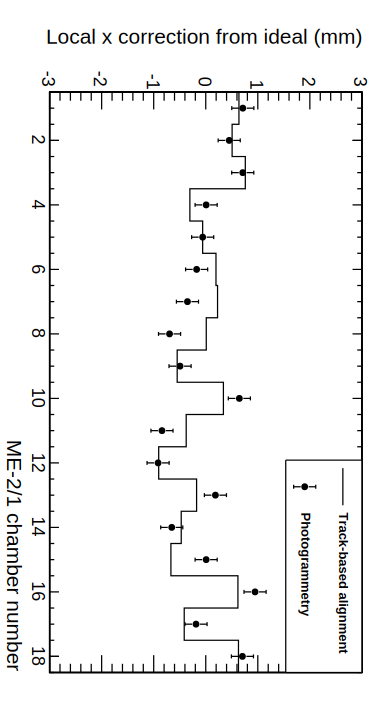
\includegraphics[height=0.45\linewidth, angle=90]{compare_m21_x.pdf} 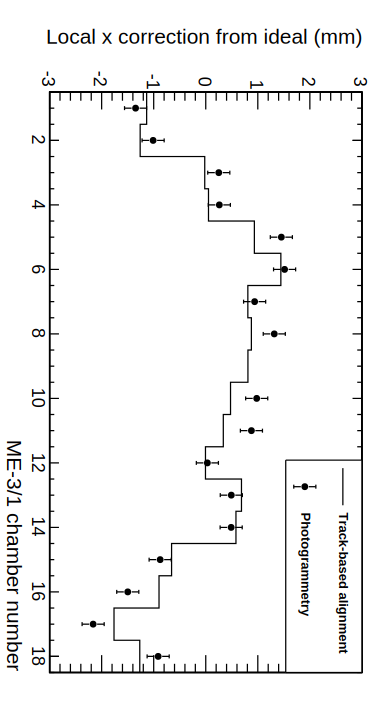
\includegraphics[height=0.45\linewidth, angle=90]{compare_m31_x.pdf}

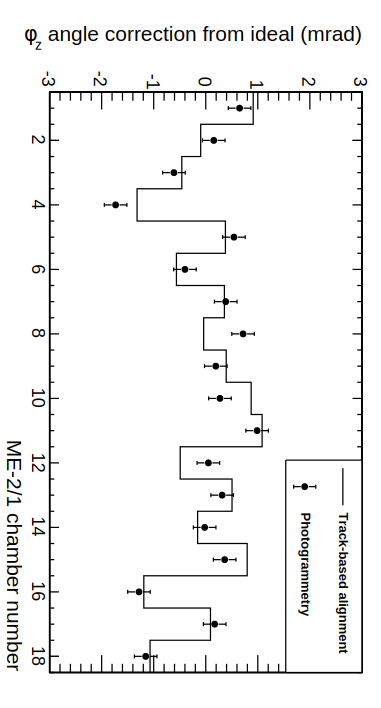
\includegraphics[height=0.45\linewidth, angle=90]{compare_m21_phiz.pdf} 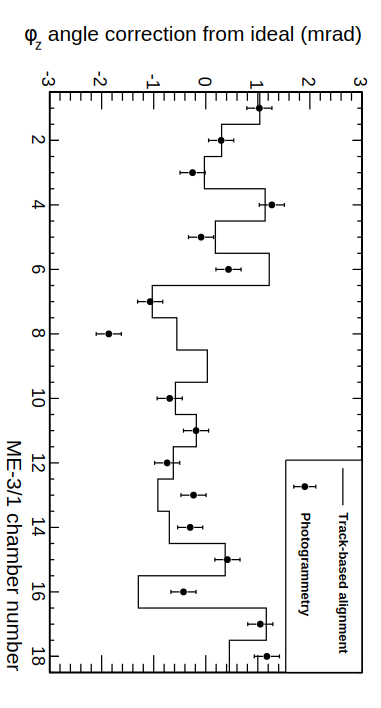
\includegraphics[height=0.45\linewidth, angle=90]{compare_m31_phiz.pdf}
\end{minipage}
\end{center}
\caption{CSC alignment results from the Overlaps procedure and the 2008 LHC run, presented as a difference from ideal and compared with photogrammetry where possible. \label{fig:overlaps_data1}}
\end{figure}

To compute the accuracy of the beam-halo alignment with photogrammetry
as the reference, we subtract the $\delta_{r\phi}$ and $\phi_z$ of
each beam-halo result from the corresponding photogrammetry result
(Fig~\ref{fig:overlaps_data2}).  The mean (bias) is consistent with
zero, but in the $\delta_{r\phi}$ case, a non-zero mean would
correspond to a global rotation of the disk which is not a measurable
parameter in the CSC Overlaps procedure or the single-disk
photogrammetry.  The standard deviations are 340~$\mu$m in
$\delta_{r\phi}$ and 0.42~mrad in $\phi_z$, which derive from a sum in
quadrature of the track-based uncertainties and the photogrammetry
uncertainties.  Photogrammetry uncertainties are 300~$\mu$m for each
pin \cite{photogrammetry}, which means $\mbox{(300~$\mu$m)}/\sqrt{2} = 210$~$\mu$m for
the chamber center position and $\mbox{(300~$\mu$m)} \cdot \sqrt{2} /
\mbox{1.85~m} = 0.23$~mrad for the chamber angle.  Subtracting the
photogrammetry uncertainties in quadrature from standard deviations
observed in the plots,
\begin{eqnarray}
\mbox{track-based $\delta_{r\phi}$ accuracy} &=& \sqrt{(\mbox{340~$\mu$m})^2 - (\mbox{210~$\mu$m})^2} = \mbox{270~$\mu$m} \\
\mbox{track-based $\phi_z$ accuracy} &=& \sqrt{(\mbox{0.42~mrad})^2 - (\mbox{0.23~mrad})^2} = \mbox{0.35~mrad}
\end{eqnarray}

\begin{figure}
\begin{center}
\includegraphics[width=0.45\linewidth]{delta_translations_goodcolors.pdf} \includegraphics[width=0.45\linewidth]{delta_rotations_goodcolors.pdf}
\end{center}
\caption{Chamber-by-chamber verification of the beam-halo alignment with photogrammetry.  The dark histogram is before alignment; the light histogram and statistics box are after alignment. \label{fig:overlaps_data2}}
\end{figure}

Thus, the 200-300~$\mu$m accuracy goals are already demonstrated in a
subset of endcap chambers, using a local alignment technique.  There
is no indication that this result is systematically limited; much
higher precision may be possible once we collect more than 12~minutes
of data.

\subsection{Extension to align CSC layers}
\label{sec:CSC_layer_alignment}

The CSC Overlaps procedure can be extended to align CSC layers, though
the layer procedure only needs to be applied once with high
statistics, rather than routinely with a maintainable algorithm.  The
usual difficulty in aligning layers with local tracks is that the
systems are underconstrained.  Extra constraints applicable to tracks
overlapping well-aligned neighbors allow us to break all of the
important degeneracies.

Local alignment procedures require tracks to be fitted locally, which
introduces an interdependency between track-fitting and alignment.  In
the CSC Overlaps procedure, we needed the circular closure constraint
to form an overconstrained system, and no such thing is available
inside of a chamber.  In a chamber, there are 6 layers; in principle,
5 need to be aligned, since the collective position of all the layers
is a chamber-alignment issue.  But it takes at least 2 parameters to
determine each track: one too many.  If we simply ignore this fact and
constrain the track to two of the layers, we would not know if the
layers are skewed like a deck of cards
(Fig~\ref{fig:layer_alignment_skew}), a plausible misalignemnt, as it
could be caused by a simple tilt of the alignment pins.  Small tilts
could also escape quality control at the production sites, which
measured cathode traces relative to the pins.

\begin{figure}
\begin{center}
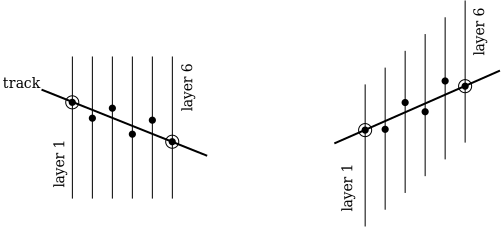
\includegraphics[width=0.75\linewidth]{layer_alignment_skew.pdf}
\end{center}
\caption{Even when a track is constrained to two only layers, the positions of the other layers can only be determined up to a collective offset and a collective skew.  The two situations depicted here are indistinguishable. \label{fig:layer_alignment_skew}}
\end{figure}

A well-aligned pair of neighboring chambers can be treated as a
single, 12-layer chamber for tracks that pass through the overlap
region.  Once misalignments between the two chambers have been
corrected with the CSC Overlaps procedure, we can justifiably assume
that the 12-layer system is not collectively skewed, and align 10 of
the layers to a track constrained to 2 layers (or an equivalent
average that maintains the same number of degrees of freedom).  Such a
procedure is illustrated in Fig~\ref{fig:layer_alignment_noskew}.

\begin{figure}
\begin{center}
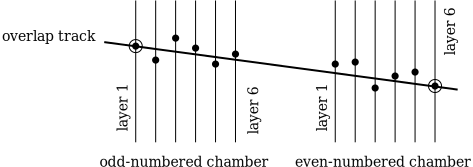
\includegraphics[width=0.75\linewidth]{layer_alignment_noskew.pdf}
\end{center}
\caption{Method for aligning layers within chambers: constrain a linear track to the first and last layers in a two-chamber overlap, then align the remaining layers to that track. \label{fig:layer_alignment_noskew}}
\end{figure}

Using beam-halo data from 2008, we applied the above procedure to
measure layer corrections in ME$-$2/1 and ME$-$3/1.  The corrections
are generally smaller than 200~$\mu$m, though some are
statistics-limited, due to the azimuthal asymmetry of the beam-halo.
They are plotted in Fig~\ref{fig:layer_hist}.

\begin{figure}
\begin{center}
\includegraphics[width=0.5\linewidth]{layer_hist.pdf}
\end{center}
\caption{Layer alignment results in ME$-$2/1 and $-$3/1, excluding layers fixed by definition. \label{fig:layer_hist}}
\end{figure}

\subsection{Verifying the global procedure with local alignment}

In addition to providing a nearly-complete alignment of the muon
endcaps before first collisions, the CSC Overlaps procedure will
diagnose the global alignment procedure.  Once collisions muons have
been collected in sufficient quantity, we will attempt to align the
CSCs with global tracks, then check it against the locally-measured
result.  If the global alignment is correct, it should reproduce the
local results, though possibly with lower precision and an overall
ring displacement, unobserved by the local measurement.

As previously stated, local track-fitting does not suffer from
potential propagation errors, and it is completely independent of any
tracker misalignments.  Overlaps tracks are a minority, so they can be
explicitly excluded from the global alignment procedure for perfect
independence.  It's also worth noting that the direction in which the
CSC Overlaps procedure correlates results, among chambers in the same
station, is orthogonal to the way global alignment correlates results,
among equal-numbered chambers in different stations.  If the global
procedure independently aligns chamber~$i$ and $i+1$ to the correct
relative values, that would be a strong confirmation.

The local alignment procedure provides a link between the global
procedure and photogrammetry.  Photogrammetry must be performed when
the magnetic field is off and disks are unbent.  The global alignment
procedure must be performed with the magnetic field on to apply an
essential $p_T$ cut; modifications of the global procedure without a
$p_T$ cut determined by track curvature would make the comparison less
meaningful.  Comparing the two is complicated by the fact that the
geometry changes when the field is turned on.  Local alignment
procedures, however, can be performed with or without the magnetic
field, because local tracks are approximately linear in either case.
We have verified that the CSC Overlaps procedure reproduces
photogrammetry with no field; what remains is to verify that the
global alignment procedure reproduces the CSC Overlaps.

If there is a discrepancy between local and global alignment results,
the similarities between the methods suggest follow-up studies.  For
instance, some tracks pass through both the tracker and the overlap
region of a CSC.  We could fit the same track both ways and look for
discrepancies on a track-by-track basis.  Studies such as these would
not be possible to diagnose differences between track-based alignment
and photogrammetry or a hardware-based alignment.

\section{Alignment outlook for 2009--2010}

This is where I will review the steps toward alignment in 2009 and
present track resolutions from the 50 and 200~pb$^{-1}$ scenarios
derived from the ``MC Results'' section.  It will be a schedule of
future tasks, a summary of the paper, and a reference for what this
alignment means for physics (Fig~\ref{fig:curvature_resolution}).

\begin{figure}
\begin{center}
\includegraphics[width=0.75\linewidth]{curvature_resolution.pdf}

\includegraphics[width=0.75\linewidth]{mass_resolution.pdf}
\end{center}
\caption{PLACEHOLDER!  Track and mass resolutions with 2008-STARTUP, 50, 200~pb$^{-1}$, and ideal scenarios from the new MC studies. \label{fig:curvature_resolution}}
\end{figure}

\begin{thebibliography}{99}

\bibitem{tdr} TDR
\bibitem{internal_dt} internal DT reference
\bibitem{photogrammetry} photogrammetry
\bibitem{SWGuideMuonGeometryConversion} {\tt https://twiki.cern.ch/twiki/bin/view/CMS/SWGuideMuonGeometryConversion}

\end{thebibliography}

\end{document}
